\chapter{Performance and optimization issues.}

	\section{Introduction.}

		Assume two data sets, as depicted in 
		Figures~\ref{fig:chap1_scatters}. Each data set has two known classes, 
		represented by asterisks and x marks. Consider that we are interested in 
		classifying new-observations of unknown data, represented by black bullet 
		marks, in either asterisks and x marks class. 
      Empirically, we may conclude that a given observation belong to the class 
		of the known  data, whose it has the \emph{closest relation}. However, 
      in same cases,  we might mislead the  classification of black bullets if the 
		relation between known and unknown data is not clear or poorly defined. 
      In order to address this issue, statistical learning provides methods 
		for modelling classification problems properly. These methods allows us to 
		define the performance targets, to grasp the main patterns from the known data, 
		and to handle the classification error.

		\begin{figure}
			\centering
			\begin{tabular}{l@{}l@{}}
		 		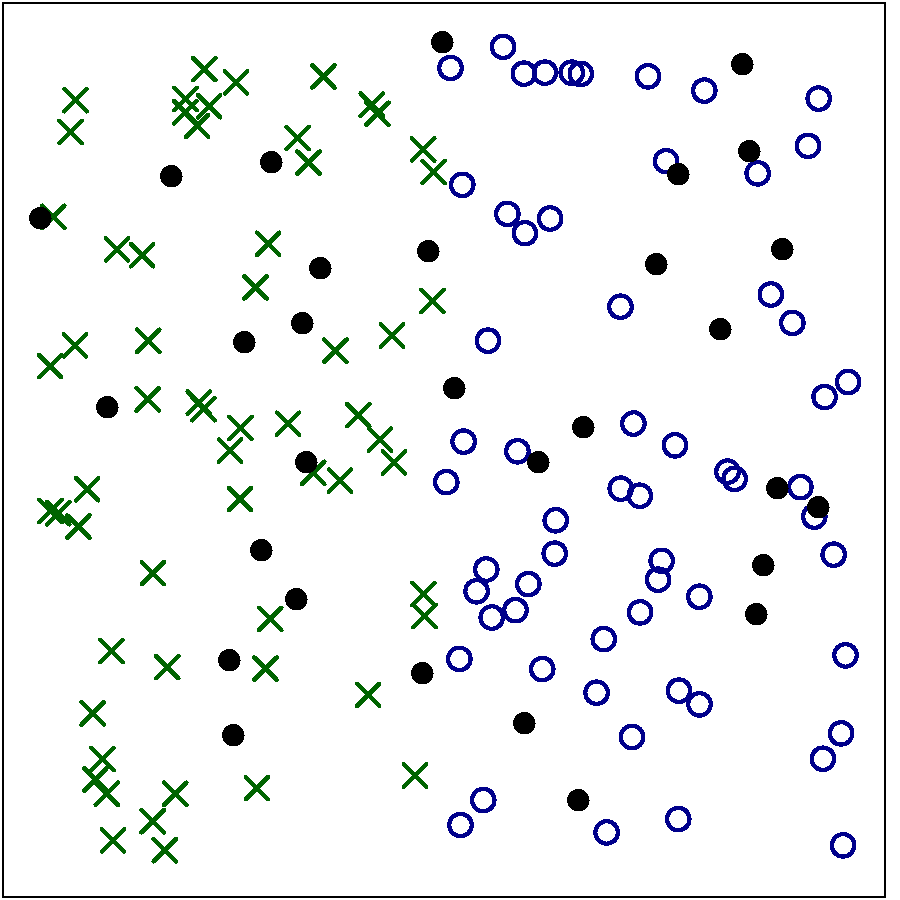
\includegraphics[width=0.45\textwidth]{inputs/img/chap1_scatter_intro_ds1} &
				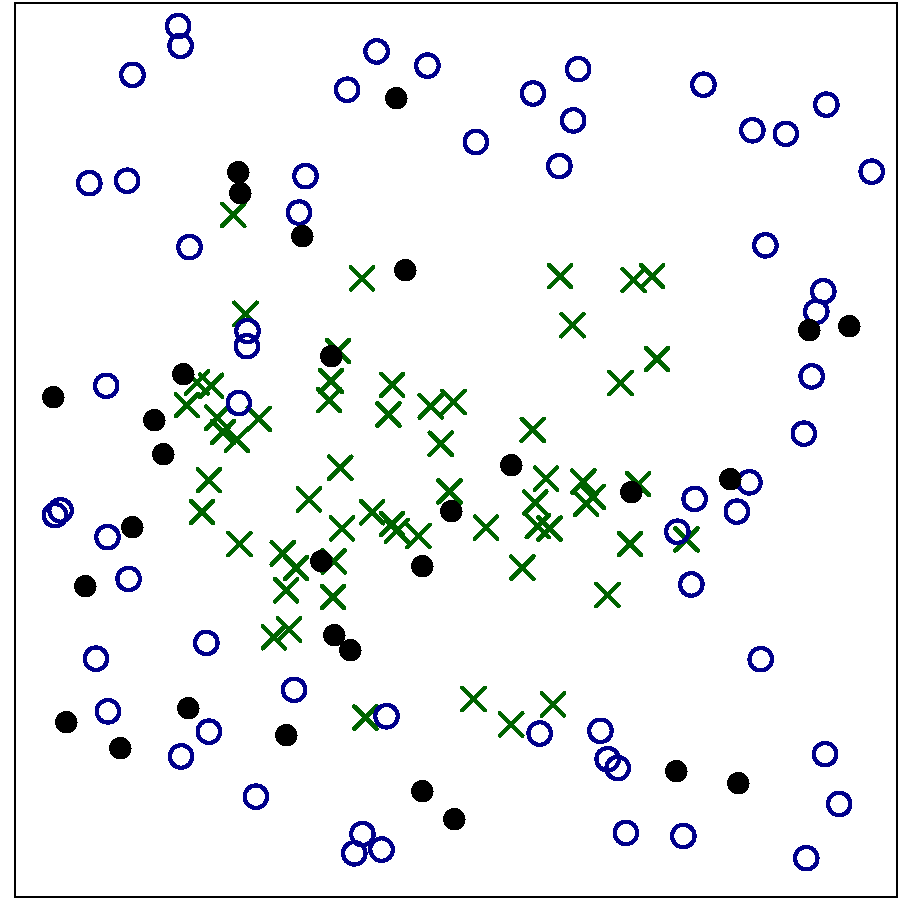
\includegraphics[width=0.45\textwidth]{inputs/img/chap1_scatter_intro_ds2} \\
			\end{tabular}
			\caption{Two classification examples in two dimensions. There are two known classes, asterisks and x marks. The problem is to classify the the unknown data, black bullets, into one of the two classes.}
		  	\label{fig:chap1_scatters}
		\end{figure}


	\section{Probabilistic model for data.}

		In this section we present our basic model. 
		
		In general, we define the law of $(X{\times}Y)$ as

		\begin{equation}
			(X,Y) \sim \mathbb{P}.
			\label{x_y_law}
		\end{equation}

		Assuming $x \in \mathcal{X}$, we can state that,

		\begin{equation}
			\mathcal{X} = \mathcal{R}^d.
			\label{x_example}
		\end{equation}

		where observations are represented by $d$-dimensional vector $x$. 

		In supervised learning, $y$ exists. It denotes the unknown nature of the observation, 
		and its characteristics depends on the classification problem. For instance,

		\begin{itemize}
			\item $|y|=2$, a binary problem, e.g. $Y = \{0,1\} \mbox{ or } \{-1,1\}.$;
			\item $|y|=K$, classification in a finite set of size K ;
			\item $y \doteq \mathbb{R}$, regression;
			\item $y = \mathbb{R}^K$, multi-task;
			\item $|y| = K$ observing the relative ordering between different values of $y$, ordinal regression.
		\end{itemize}
		
		\subsection{Definition of the law of $\mathbb{P}$.}

			We present two definitions of $\mathbb{P}$:

			\begin{enumerate}[a)] % a), b), c), ...
				\item Generative definition.
					\begin{equation}
						\mathcal{L}(X,Y) \equiv \mathbb{P} \leftrightarrow (\mathcal{Y}(Y), \mathcal{Y}(X|Y)).
						\label{p_generative_law_example}
					\end{equation}
				e.g. for $y=\{-1,+1\}$\\ 
				\centerline{$\mathcal{L}(X|Y) \leadsto (\mathbb{P}_{+},\mathbb{P}_{-})$}

				considering $\mathcal{L}(X|Y) \leadsto \mathcal{L}(X)$, and $(\mathbb{P}_{+},\mathbb{P}_{-}) \leadsto \mathcal{Y}(X|Y_{=+1})$, we have\\ 
				\centerline{$\mathbb{P}_X = _{P}\mathbb{P}_{+} + _{1-P}\mathbb{P}_{-}$}


				\item Alternative definition through a \emph{posteriori probability} function \cite{tc_Lugosi} (so-called ``dissertatif'' in french).
					\begin{equation}
						\mathcal{Y}(X,Y) \equiv (\mathcal{L}(X)\mathcal{L}(Y|X)).
						\label{p_generative_law_example}
					\end{equation}
			\end{enumerate}
			so that\\
			\centerline{$\forall x \in, \eta(x)=\mathbb{P}(Y=1|X=-1)$}
			Here, $\eta(x)$ represents the state of $X$.
		


	\section{Prediction problem statement.}
		
		\subsection{Types Prediction problems.}
			Based on the learning scenario, we can list predictions problems as follows:
	
			\begin{itemize}
				\item Classification: 
					\begin{itemize}
						\item classification data: $|y|<+\infty$; 
						\item goal: predict a new $x$.
					\end{itemize}
				\item Scoring or bipartite raking: 
					\begin{itemize}
						\item classification data: $|y|<+\infty$; 
						\item goal: ordering a new bunch of $X$, $(x_1,x_2,\dots,x_m)$, taking into account the state of $x$, where $\eta(x)=\mathbb{P}(Y=1|X=x)$. An remarkable example of this kind of problem is the ranking mechanism of search engines.
					\end{itemize}
				\item Raking: 
					\begin{itemize}
						\item data features: e.g. $|y|=\{1,2,3\}$, where $1 \ll 2 \ll 3$;
						\item goal: ordering a new bunch $x$.
					\end{itemize}
				\item Preference learning: 
					\begin{itemize}
							\item $(X,X')$, and $sign(y-y')$
						\item goal: binary classification $(X,X'_Z)$, where $Z \in \{-1,1\}$.
					\end{itemize}
			\end{itemize}

		\subsection{How to approach a prediction problem.}
			\begin{itemize}
				\item Define the performance goal $R$. 
				\item Select the set of predictors $\mathcal{F}$. Examples: 
					\begin{itemize}
							\item Binary classification: $\mathnormal{f}:\mathbb{R}^d\rightarrow\{-1,1\}$
							\item Scoring: $\mathnormal{f}:\mathbb{R}^d \times \dots \times \mathbb{R}^d \rightarrow {\sigma}_m $ (permutation  of $m$ elements/vectors);
							\item Preference function: $\mathnormal{f}:\mathbb{R}^d \times \mathbb{R}^d \rightarrow \{-1,1\} \mbox{ or } \{-1,0,1\}.$
					\end{itemize}
			\end{itemize}

		\subsection{Performance/error issues.}

			Lets define

			\[ \forall x \in, \mathnormal{f}, R(f)=\mathbb{E}[l(Y,f(x))] =  \int_{x{\times}y} f(x)\,dP(x,y).\] 

			where $l:y{\times}y \rightarrow \mathbb{R}^d$ is the measure of \emph{loss} or \emph{error}.
			
			Examples of loss:
					\begin{itemize}
							\item Binary classification: $l(y,f(x)) = 1|\{y \neq f(x)\}$.
							\item Regression: $l(y,f(x))=(y_f(x))^2$.
							\item Optimization issue: $l(y,f(x))=(1-yf(x))_+ = \Phi(yf(x))$.
							\item Log likelihood: $l(f(x))=\ln(f(x))$.
					\end{itemize}

	\section{Example: supervised classification}
		%\subsection{} 
